\chapter{Literature Review}
In section 2.1, some theories related to imbalanced datasets are described, including their importance, the impact of imbalanced medical datasets, and a review of related works that focused on imbalanced medical datasets. This section highlights the gaps in the works on imbalanced data classification if only general classification algorithms are used. It is followed by the section 2.2 which includes the methods of dealing with imbalanced classification in detail from three perspectives and several state-of-the-art and classical algorithms for imbalanced classification are introduced and explained. At the end of this chapter, in section 2.3, several metrics applied for evaluating the imbalanced classification models are briefly described. 

\section{An Overview of Theory Related to Imbalanced Medical Datasets}
\begin{figure}[h]
    \centering 
    \begin{minipage}{0.45\textwidth}
        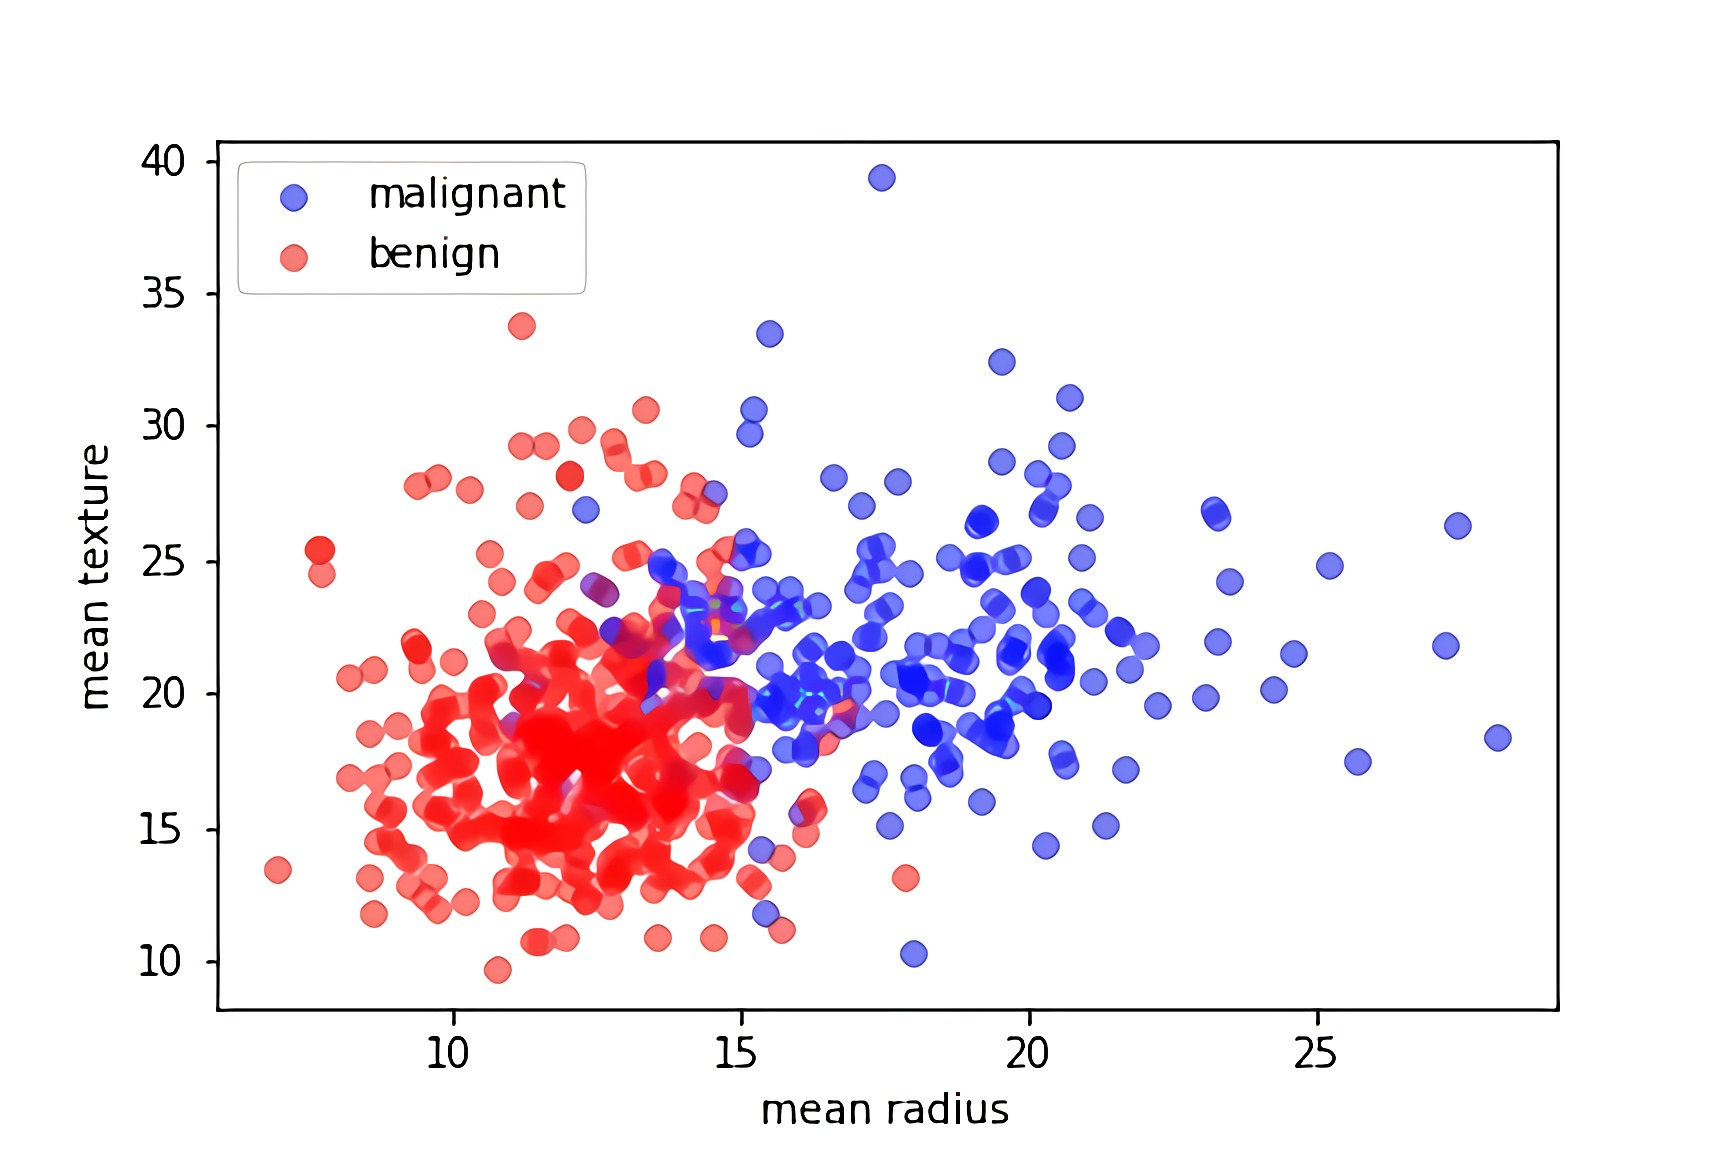
\includegraphics[width=\textwidth]{images/fig1}
        \caption{Class distribution on the dataset with IR=1.684}
        \label{fig1}
    \end{minipage}
    \quad
    \begin{minipage}{0.45\textwidth}
        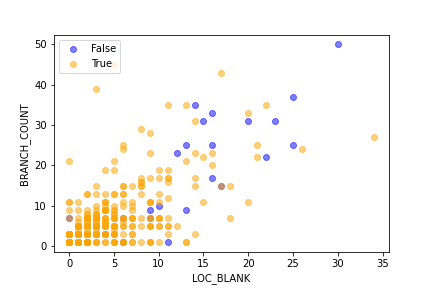
\includegraphics[width=\textwidth]{images/fig2}
        \caption{Class distribution on the dataset with IR=12}
        \label{fig2}
    \end{minipage}
\end{figure}

The class imbalance problem means one class contains a small number of data instances, but the other one is represented by a large number of data instances \cite{10}. In practical situations, the ratio between these two classes may be substantial, similar to 1:100, 1:1000, 1:10000, or even higher \cite{1}. Figure \ref{fig1} and Figure \ref{fig2} show the difference between two datasets with an  Imbalance Ratio(IR) of 12 and 1.684,  respectively. In addition, it should be noted that, under some specific circumstances, the problem of class imbalance has an internal cause \cite{1}. For example, Haibo He and Edwardo A. Garcia gave an example of cancer classification in their 2009 work \cite{17}. Such an example demonstrates that, in the screened population, the prevalence of cancer is particularly low, which leads to the class imbalance problem in the collected data, in which one disease state is underrepresented \cite{17}. However, due to the limitation of the data collection process, in areas where there is no inherent imbalance, there is also the possibility for the occurrence of a class imbalance problem: namely, the way of choosing the data by researchers (for example which data and in what quantity) and the imbalanced cost for different errors can also lead to class imbalance problems \cite{1}. Such a situation may vary from case to case \cite{1}. Affected by these conditions, normal classifiers are often confused by the majority class and ignore the minority class \cite{1}. Additionally, for the percentage of examples available for each class, most real-world data processed using non-linear classification strategies are imbalanced, which may cause the algorithm to learn overly complicated models that overfit the data and have almost no correlation \cite{2}. This issue is critical since it leads to a significant barrier in the performance achieved by basic learning methods which assume that the class distribution is balanced \cite{2}.

Classification in medical diagnostics can aid in disease diagnosis and predict outcomes in response to treatment \cite{3}. For instance, with Computer Aided Decision(CAD) systems, a physician is able to diagnose a patient with the help of computer algorithms and classification is one of the most common tasks performed by the CAD system \cite{4}. However, data collection in the medical sector is associated with a number of challenges and practical limitations. The collection of patient data is time-consuming \cite{4} and the collection of balanced model training data is difficult where there is low prevalence of the disease \cite{7}. In addition, the inherent heterogeneity, incompleteness, and high-dimensional nature of healthcare/medical data can also lead to challenges \cite{5}. The medical data is often heterogeneous where patient records contain various data types, including images, real and integer with different ranges, and text types \cite{5}.

Many classification algorithms have been developed recently and used to detect and predict some common diseases such as diabetes, Parkinson's disease and vertebral column pathologies, which has brought significant trouble and pain to a tremendous number of patients \cite{6}.

Study \cite{5} addressed the problems of imbalanced healthcare data on the diagnosis of a brain tumor. In this study, a new approach to data mining is adopted, combining feature selection and ensemble classification. Study \cite{3} introduced a novel voting class weight algorithm called CWsRF based on random forest algorithm (RF), which focuses on the challenge of identifying the minority class sufficiently in medical applications and can be applied to the detection of diseases, such as breast cancer, or medical images classification. Study \cite{8} offers an innovative ensemble learning paradigm for the early detection of diseases with imbalanced data that functions equally as well as or outperforms the other state-of-the-art comparison algorithms, such as support vector machines and random forest. This algorithm is the first comprehensive ensemble learning technique that involves multiple SVM diversity structures for classification, which can prevent the generation of noisy instances and effectively re-balance the input data \cite{8}. 

\section{Related Work on Imbalanced Classification}
\subsection{Sampling Methods}
Resampling, which involves creating a new transformed version of the training set of an imbalanced dataset, offers a set of practical and straightforward approaches to provide a more balanced data distribution \cite{9}. All these approaches can be classified into three groups: Oversampling techniques, Undersampling techniques, and Hybrids techniques \cite{10}. In the first case, oversampling, the original dataset will be augmented by replicating the selected instances or creating new instances from the existing one, while with undersampling methods, a set of data (usually majority class samples) will be removed from the original set. The hybrid methods are a combination of both from sampling algorithms \cite{10}. Among these three groups, random oversampling and random undersampling are non-heuristic and the simplest approaches; the former case has the drawback of overfitting, and in the case of the latter, the omission of some crucial samples pertaining to the majority class may occur due to the removal of examples \cite{17}. Moreover, informed undersampling based on the traditional undersampling method aims to deal with information loss deficiency. The \textit{EasyEnsemble} and \textit{BalanceCasade} are two applications of this algorithm with good performance \cite{12}. Additionally, synthetic sampling with data generation is also a useful approach to improve data distribution. Some of the renowned algorithms in this area are the \textit{SMOTE} \cite{13} and the \textit{Borderline-SMOTE} \cite{15}, which was applied to various situations with a great deal of success. In addition, to deal with the overlapping introduced from sample methods, data cleaning techniques have been used practically \cite{17}. \textit{Tomek links} \cite{16} is representative of this kind of method. 

\subsection{Cost-Sensitive Learning Methods}
Sampling methods try to improve the balanced level of the dataset, while cost-sensitive learning methods are utilized to deal with different misclassification errors that incur different penalties to find the optimal decision. The foundation of these decisions is the cost matrix, which is fundamental to the cost-sensitive learning methodology \cite{17,18}. Table \ref{tab1} illustrates the structure of a binary classification cost matrix. The positive category (class label 1) denotes the minority and the negative category (class label 0) represents the majority. If $m$ stands for the predicted label and $n$ stands for the actual label, so the $C(m, n)$ is the cost of predicting a class $n$ sample as class $m$. For example, $C(1,0)$ represents the cost of predicting a negative instance as positive. In view of the cost matrix, the purpose of this type of learning method is explained to create a model with minimal overall misclassification costs \cite{19,20}.
\begin{table}[h]
    \centering
    \begin{tabular}{|c|c|c|}
    \hline
                     & Actual negative & Actual positive \\ \hline
    Predict negative & $C(0,0)$        & $C(0,1)$        \\ \hline
    Predict positive & $C(1,0)$        & $C(1,1)$        \\ \hline
    \end{tabular}
    \caption{Cost Matrix for Binary Classification}
    \label{tab1}
\end{table}

Bearing in mind most traditional classifiers assume that the misclassification has the same cost for false negative(FN) and false positive(FP) \cite{18}. However, real-world scenarios are not so ideal. Conceptually, in certain situations, the cost of incorrect labeling for a sample should always be higher than a correct one \cite{18}. For instance, in cancer diagnosis, where a patient who does have a certain kind of cancer is classified as negative(FN), this error could be much more serious and expensive than regarding a non-cancer patient as positive(FP), which can be corrected by further medical examinations; the former situation may lead to a worse patient condition or the even more severe outcome of losing his life \cite{21}. In another scenario, the cost of not mailing to potential buyers is higher than mailing to some non-buyers  \cite{19}. From this, it can also be illustrated that costs are not necessarily only monetary but also can be the severity of an illness or the wasting of time \cite{18}. 

The cost matrix values should be defined with care because the supplied cost matrix can strongly impact effectiveness \cite{10}. However, in many cases, the cost of classification errors cannot be described clearly. The determination of a given domain's cost representation can be a challenge and, under some circumstances, impossible \cite{17}. There may be a problematic accession to a domain expert or a lack of available prior information on the cost matrix during the classifiers' training process, which is a common phenomenon when cost-sensitive learning is utilized to deal with the class imbalance problem \cite{10}. 

Cost-sensitive learning techniques can be categorized into two families: \textit{Meta-learning} (including two aspects: thresholding and sampling) and \textit{Direct methods} \cite{20}. The principle of the former category is to create a ``wrapper'' to turn existing cost-insensitive classifiers into cost-sensitive classifiers, and in the latter case, classifiers that are cost-sensitive in themselves are constructed \cite{20}. 

The \textit{cost-sensitive decision trees} which have taken account of misclassification during pruning are popularly used as direct methods for detecting card fraud when the cost to misclassify could vary \cite{20,22}. \textit{MetaCost} \cite{23} can be viewed as a representative thresholding tool in the case of thresholding. \textit{Weighting} \cite{24} is one implementation of the sampling methods, in which examples of the minority are assigned high weights according to their proportion.

\subsection{Ensemble Learning Methods}
In 2004, a statistician named James Michael Surowiecki presented in his study \cite{34} that, under certain controlled circumstances, the decisions or predictions made by groups of humans often outperform those made by a single individual. 

The ensemble methodology is used in classification to enhance the output of an individual classifier, which is likely to ask multiple ``experts'' for help: the key idea is to train multiple classifiers and then combine them to achieve an overall classification that overtakes each indivudual classification to produce the final decision \cite{26}. Therefore, the predictions of all members of this ensemble, known as classifier fusion or aggregation are considered in the combining step, in order to classify a new unknown example \cite{10}. In 1979, Dasarathy and Sheela proposed one of the earliest work on ensemble learning \cite{30}. In \cite{30}, the partition of the feature space with two or more classifiers was discussed. Later in 1990, Hansen and Salmon introduced the idea that \textit{ensemble artificial neural networks (ANNs)} with similar configurations can improve a single classifier's generalization performance \cite{31}. Furthermore, the ensemble learning approach was successfully applied to various industries, including medical diagnosis \cite{27}, cheminformatics \cite{28}, bioinformatics \cite{29} and so forth. \textit{Bagging and Boosting} are the two most practical techniques of ensemble learning, which apply instance partitioning methods \cite{36}.

\textit{Bagging} is the abbreviation of Bootstrap Aggregating introduced by Breiman in 1996 \cite{37}, which is a simple but successful method for building a set of classifiers that are suitable not only for dealing with binary, but also multi-class classification \cite{26,33}. In detail, every single classifier in the ensemble is trained on a set of examples which are taken with replacement from the training set \cite{26,33,37}. The base classifier can be trained by using the base learning approach with each set \cite{33}. Major voting is used to generate the ultimate prediction for the composite bagging classifier \cite{26}. Study \cite{33} indicates that, due to the generation of data samples with the bootstrap sampling \cite{37}, there is a large overlap among all data samples. A stable learner (a base algorithm that is intensive to perturbation on training sets) may lead to a set of classifiers whose predictions are very similar with no improvement in generalization after the combination \cite{26,33}. Therefore, a relatively unstable learner should be utilized to ensure the diversity among the ensemble classifiers under this scenario so that sufficiently different decision boundaries can be obtained for small perturbations in different training sets. Random Forests \cite{39} is an extension of the bagging algorithm generated from individual decision trees, whose specific training parameters that can be bootstrapped replicas of the training data, as in bagging, vary randomly \cite{38}.

The word \textit{boosting} refers to a group of algorithms which can transform weak learners (an algorithm generating classifiers that outperform random guessing) to strong learners(low error with high confidence for all class concepts), proven by Schapire in his 1990 study \cite{40}. Similar to Bagging, boosting also generates an ensemble classifier by applying resampling methods on data and is later combined with major voting \cite{26,38}. Freund and Schapire introduced one of the representative works of boosting in 1997, named \textit{AdaBoost}(Adaptive Boosting) \cite{41}, which applies an iterative process to simple boosting in order to improve performance. This approach focuses on the instances which are much more complex to classify. To be clear, in \textit{AdaBoost}, a new dataset, in which more weight is assigned to the instances that are misclassified by the previous classifier and less weight is assigned to the one with a correct prediction, is used for training each subsequent classifier \cite{42}.

\subsection{An Overview of Algorithms on Imbalanced Classification}
\subsubsection{Classical Imbalance Classification Algorithms}
\textbf{\textit{Synthetic Minority Oversampling Technique(SMOTE)}} \cite{13} addresses the class imbalance problem by generating synthetic samples in feature space (Fig \ref{fig3} SMOTE working procedure illustrates the detail of this procedure). One minority class example $s_{1}$ will be selected randomly and then its $k$ nearest neighbors in minority class will be screened out; a line segment is formed between one of these $k$ neighbors $s_{2}$, which is selected at random, and $s_{1}$ in the feature space \cite{13}. SMOTE creates the synthetic samples through a convex combination of $s_{1}$ and $s_{2}$ \cite{51}. As described in \cite{61}, random undersampling is suggested to be used to curtail the size of the majority in the first instance. Next, \textit{SMOTE} is utilized on the training set to align the class distribution. This approach combined with random undersampling is proven to outperform the plain undersampling \cite{13}. 
\begin{figure}[h]
    \centering
    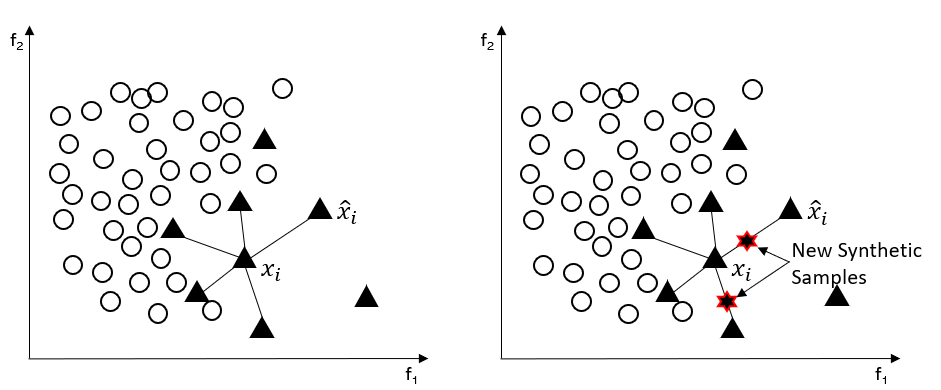
\includegraphics[width=\textwidth]{images/fig3}
    \caption{SMOTE working procedure \cite{100}}
    \label{fig3}
\end{figure}

\textbf{\textit{AdaBoost}} \cite{63} is a boosting ensemble learning approach utilized to deal with the class imbalance problem; the key principle behind it is to enhance the weak learner gradually into a strong learner. This is implemented by varying the sample weight, which indicates its importance in the classifier training process, stage by stage. Fig \ref{fig4} shows the process of combining the ultimate classifier.
\begin{figure}[h]
    \centering
    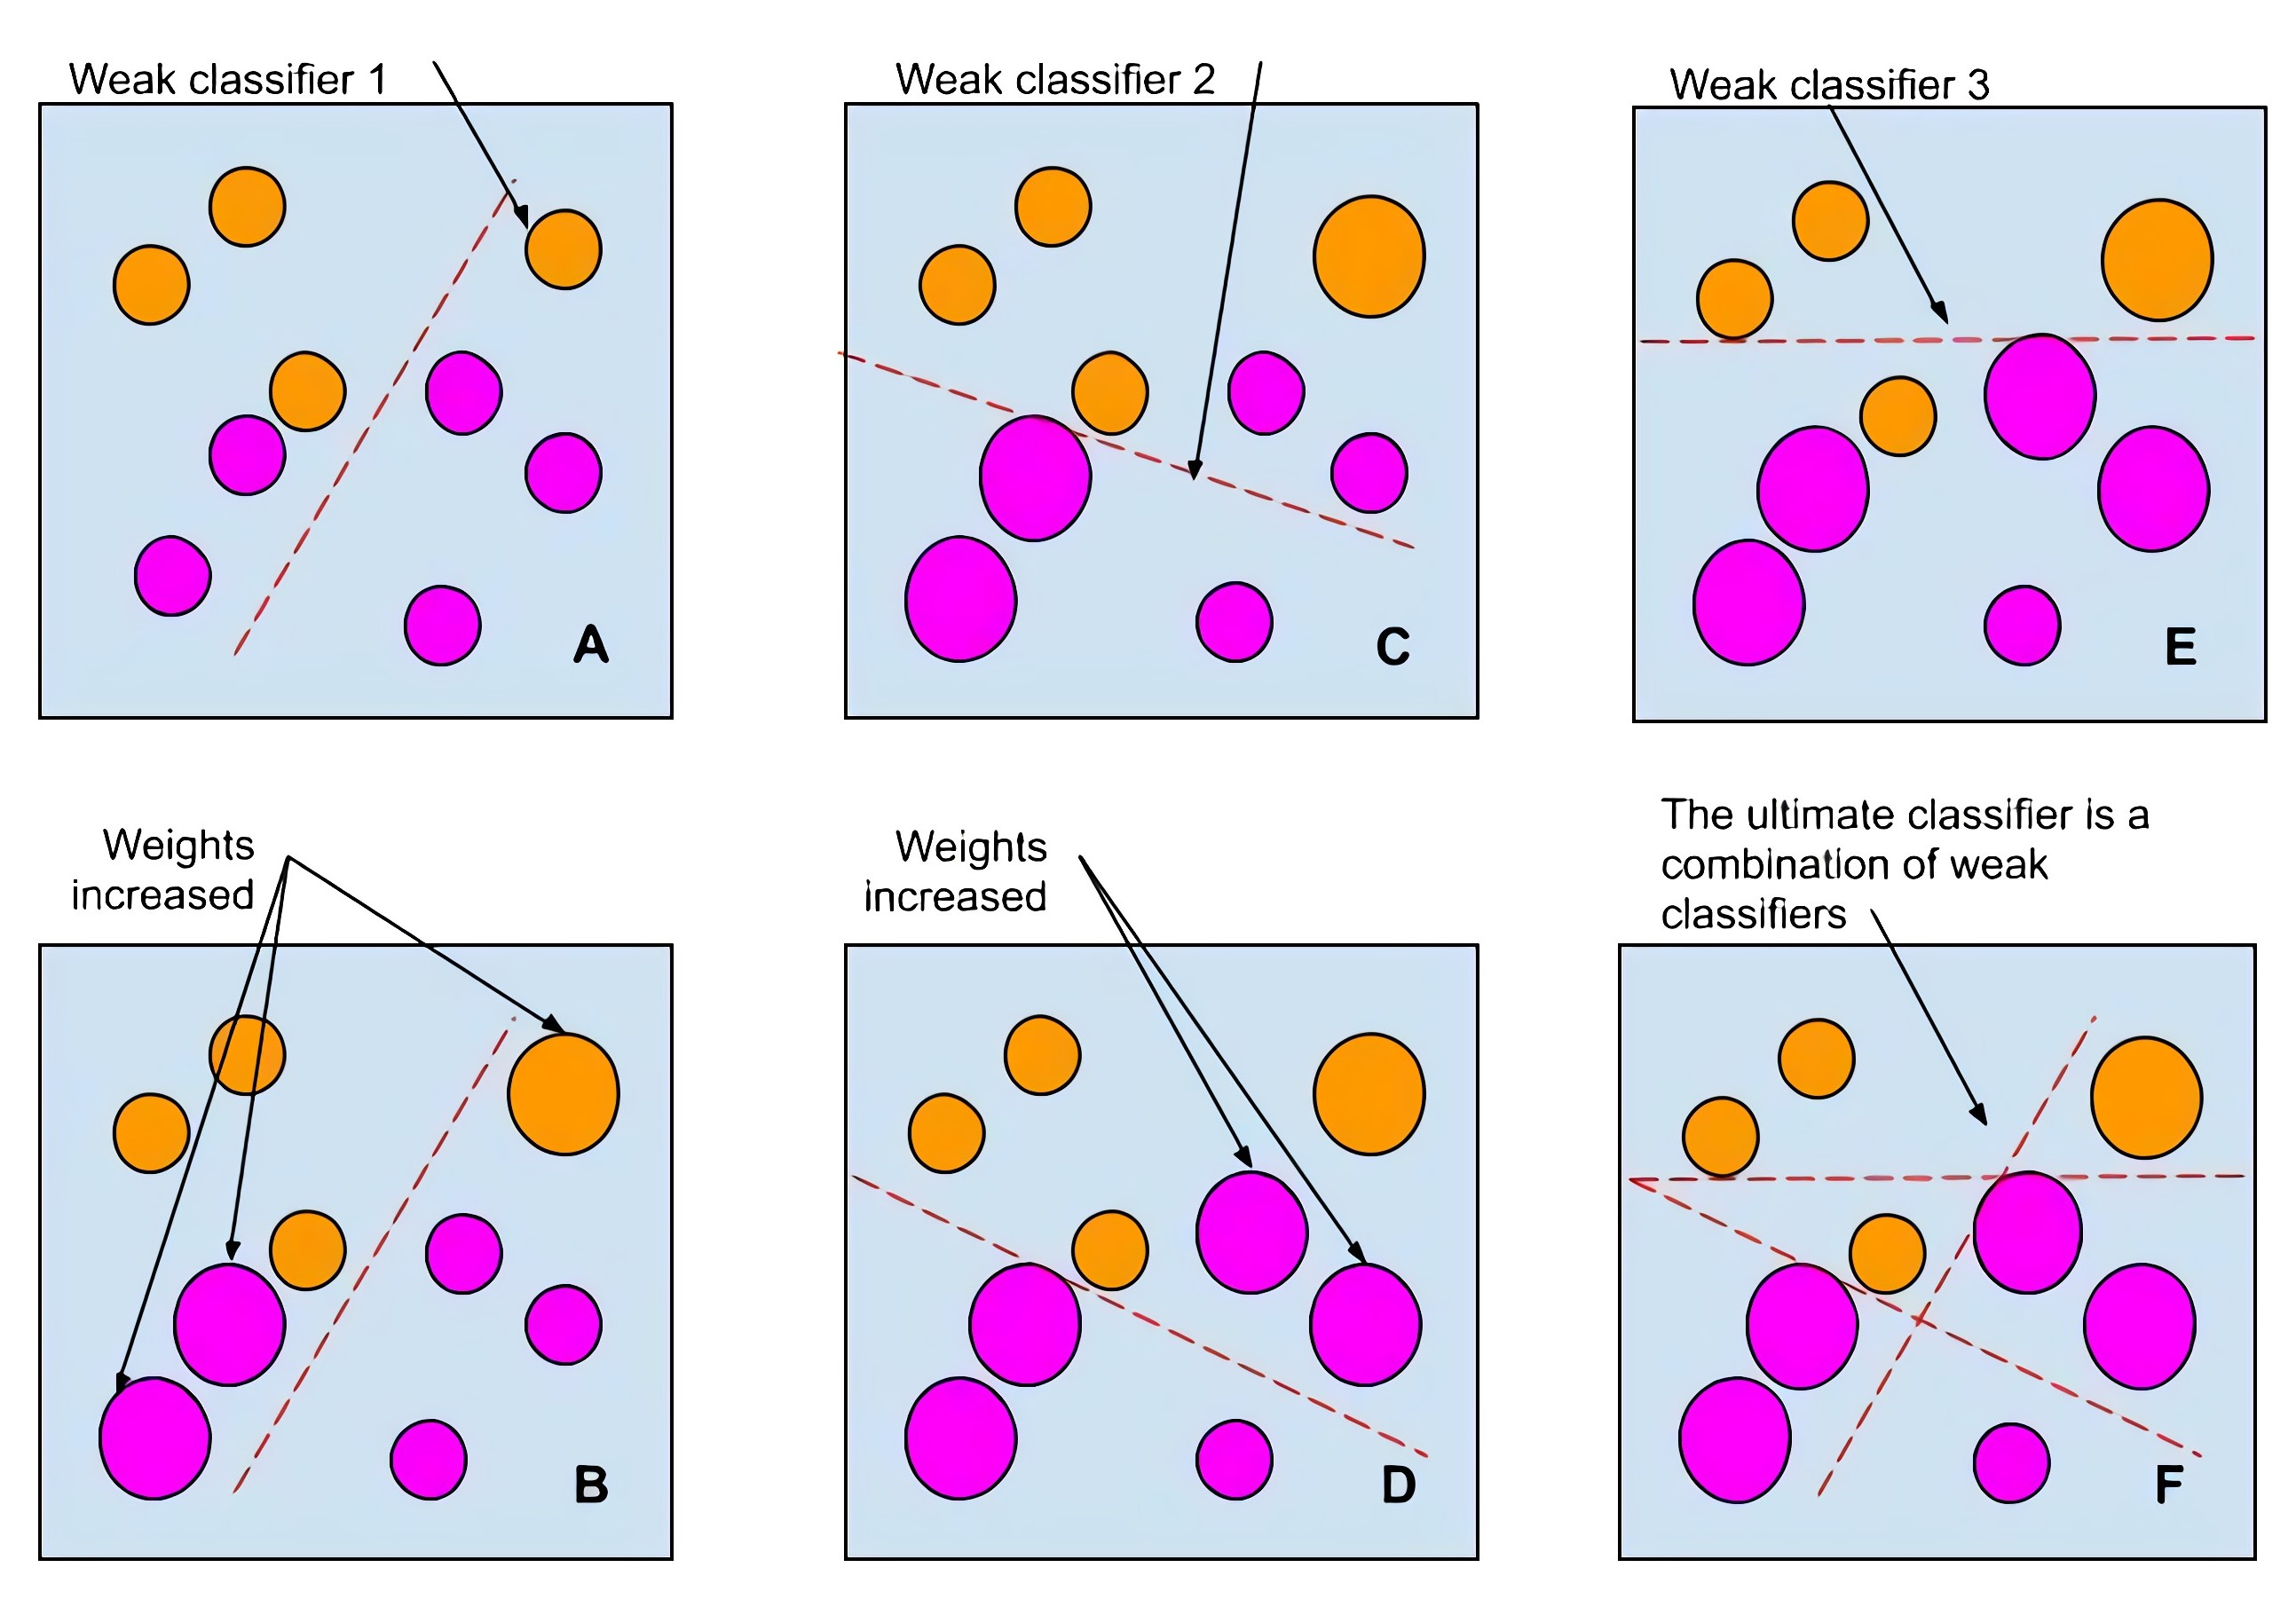
\includegraphics[width=\textwidth]{images/fig4}
    \caption{The process of the combination of the ultimate strong learner in \textit{AdaBoost}}
    \label{fig4}
\end{figure}

\textbf{\textit{Majority Weighted Minority Oversampling Technique (MWMOTE)}} \cite{62} balances the class distribution also by generating synthetic examples. Unlike SMOTE, this approach creates synthetic examples from a weighted minority class through a clustering approach; and the weight of each important minority sample is chosen on the basis of its Euclidean distance to the nearest majority class sample \cite{62}.

\textbf{\textit{RUSBoost}} \cite{64}, a combination of data sampling and boosting algorithm, is based on \textit{SMOTEBoost} \cite{68} that balances class distribution through \textit{SMOTE} and works on improving classifier performance with the balanced data under the help of \textit{AdaBoost}.  Instead of \textit{SMOTE}, this hybrid approach utilizes random sampling(RUS) to achieve increased performance \cite{64}.

\textbf{\textit{CAdaMEC}} \cite{67} is proposed upon \textit{AdaMEC} \cite{66}(a cost-sensitive algorithm) through an appropriate calibration with Platt scaling.

\textbf{\textit{MetaCost}} \cite{23} is one of cost-sensitive learning models through wrapping a cost-minimizing method, which has no restriction on the number of classes or arbitrary cost matrices. This procedure relabels the instances in the training set with the class labels that have estimated minimal-cost, then the new replacement training set will be applied to the error-based learners \cite{23}.

The principle of \textbf{\textit{cost-sensitive decision tree(csDCT)}} is to consider minimizing two separate costs: the test cost of the \textit{i}th feature and the cost of misclassification of the sample \cite{10}.

\subsubsection{Recent State-of-the-art Imbalance Classification Algorithms}
\textbf{\textit{Self-paced Ensemble Classifier}} \cite{96} is an effective ensemble classifier generated by self-paced harmonizing data hardness through undersampling. It has been proven that this model can achieve robust performance even when the classes are highly overlapped and the data distribution highly skewed \cite{96}.

\textbf{\textit{DDAE}} \cite{73} is a novel model to address the class imbalance problem consisting of several classical approaches, including resampling, data metrics learning, cost-sensitive-learning, and ensemble learning. More detail will be described in section 3.2.1.

\textbf{\textit{Iterative Metric Learning (IML)}} \cite{72} focuses on the exploration of a stable neighborhood space for each of the data samples in the testing set. To achieve this, the proposed procedure utilizes an iterative metric learning technique \cite{72}. More detail will be described in section 3.2.2.

\section{Evaluation Metrics for Imbalanced Classification}
Evaluation of classification performance always plays a significant role in guiding and learning performance \cite{44}. \textbf{\textit{Confusion matrix}} \cite{104} provides a deeper understanding of predictive model performance through the results of the predictions so that the types of error can be more clearly observed. Table \ref{tab2} shows the structure of a confusion matrix for binary classification. Table \ref{tab3} shows the measures derived using the confusion matrix from Table \ref{tab2}
\begin{table}[h]
    \centering
    \begin{tabular}{|c|c|c|}
    \hline
                     & Actual negative                              & Actual positive                              \\ \hline
    Predict negative & \textit{TN}(True Negative)  & \textit{FN}(False Positive) \\ \hline
    Predict positive & \textit{FP}(False Positive) & \textit{TP}(True Negative)  \\ \hline
    \end{tabular}
    \caption{Confusion Matrix for Binary Classification}
    \label{tab2}
\end{table}

Cesar Ferri et al. categorized evaluation metrics into three groups in their 2008 work \cite{45}: \textit{probability metrics}, \textit{ranking metrics} and \textit{threshold metrics}. In this paper, two groups of metrics, threshold and ranking metrics, are applied to evaluate the model performance.

Thresholding metrics, which quantify the classification prediction error, focuses on the generalization ability of the trained classifier through the quality of the trained classifier when used to predict unknown examples \cite{46}. The most common threshold metric is the \textbf{\textit{accuracy}} of classification applied in most conventional applications; nevertheless, accuracy is inappropriate for evaluating the imbalanced dataset since it is simple for a classifier that only predicts the majority to yield a low error \cite{47}. 

Sensitivity-specificity metrics are practical thresholding metrics for imbalanced classification that are applied by several researchers \cite{49,50}. As defined in Table \ref{tab3}, \textbf{\textit{specificity}} means the true negative rate. \textbf{\textit{Sensitivity}}, the complement to specificity, describes the true positive rate. The \textbf{\textit{geometric mean (G-mean)}} calculated through the combination of sensitivity and specificity, which has been used by Kubat and Matwin in their 1997 paper \cite{58}, can balance both concerns. Sensitivity, Specificity and G-mean are taken into account when both positive and negative classes are meaningful at the same time \cite{48}. In addition, Precision-Recall metrics arising from the fields of information retrieval are utilized when the output of the minority(class positive) is more crucial \cite{52}. In this paper, \textbf{\textit{F1}} (the value of $\beta$ in $F_{\beta}$-\textit{Measure} is 1) is utilized as one of the most important evaluation metrics.
\begin{table}[h]
    \centering
    \renewcommand\arraystretch{2.5}
    \begin{tabular}{|m{0.3\textwidth}<{\centering}|m{0.6\textwidth}<{\centering}|}
    \hline
    Metrics                       & Formula                                                                                                                                 \\ \hline
   \textit{Accuracy}             & $\dfrac{T P+T N}{T P+T N+F P+F N}$                                                                                             \\ \hline
    \textit{Error Rate}           & $\dfrac{F P+F N}{T P+T N+F P+F N}$                                                                                             \\ \hline
    \textit{Precision}            & $\dfrac{T P}{T P+F P}$                                                                                                         \\ \hline
    \textit{Recall (Sensitivity)} & $\dfrac{T P}{T P+F N}$                                                                                                         \\ \hline
    \textit{$F_{\beta}$-Measure}  & $\dfrac{\left(1+\beta^{2}\right) * \text { Precision } * \text { Recall }}{\beta^{2} * \text { Precision }+\text { Recall }}$ \\ \hline
    \textit{Specificity}          & $\dfrac{T N}{T N+F P}$                                                                                                         \\ \hline
    \textit{Geometric Mean}       & $\sqrt{\text { Sensitivity } * \text { Specificity }}$                                                                         \\ \hline
    \end{tabular}
    \caption{Evaluation Metrics based on Confusion Matrix}
    \label{tab3}
\end{table}

Nonetheless, threshold metrics are not suitable when the distribution of categories observed in the training dataset does not match the distribution of the test set and the actual data, which can make the performance misleading \cite{51}. 
\begin{figure}[h]
    \centering
    \begin{minipage}{0.49\textwidth}
        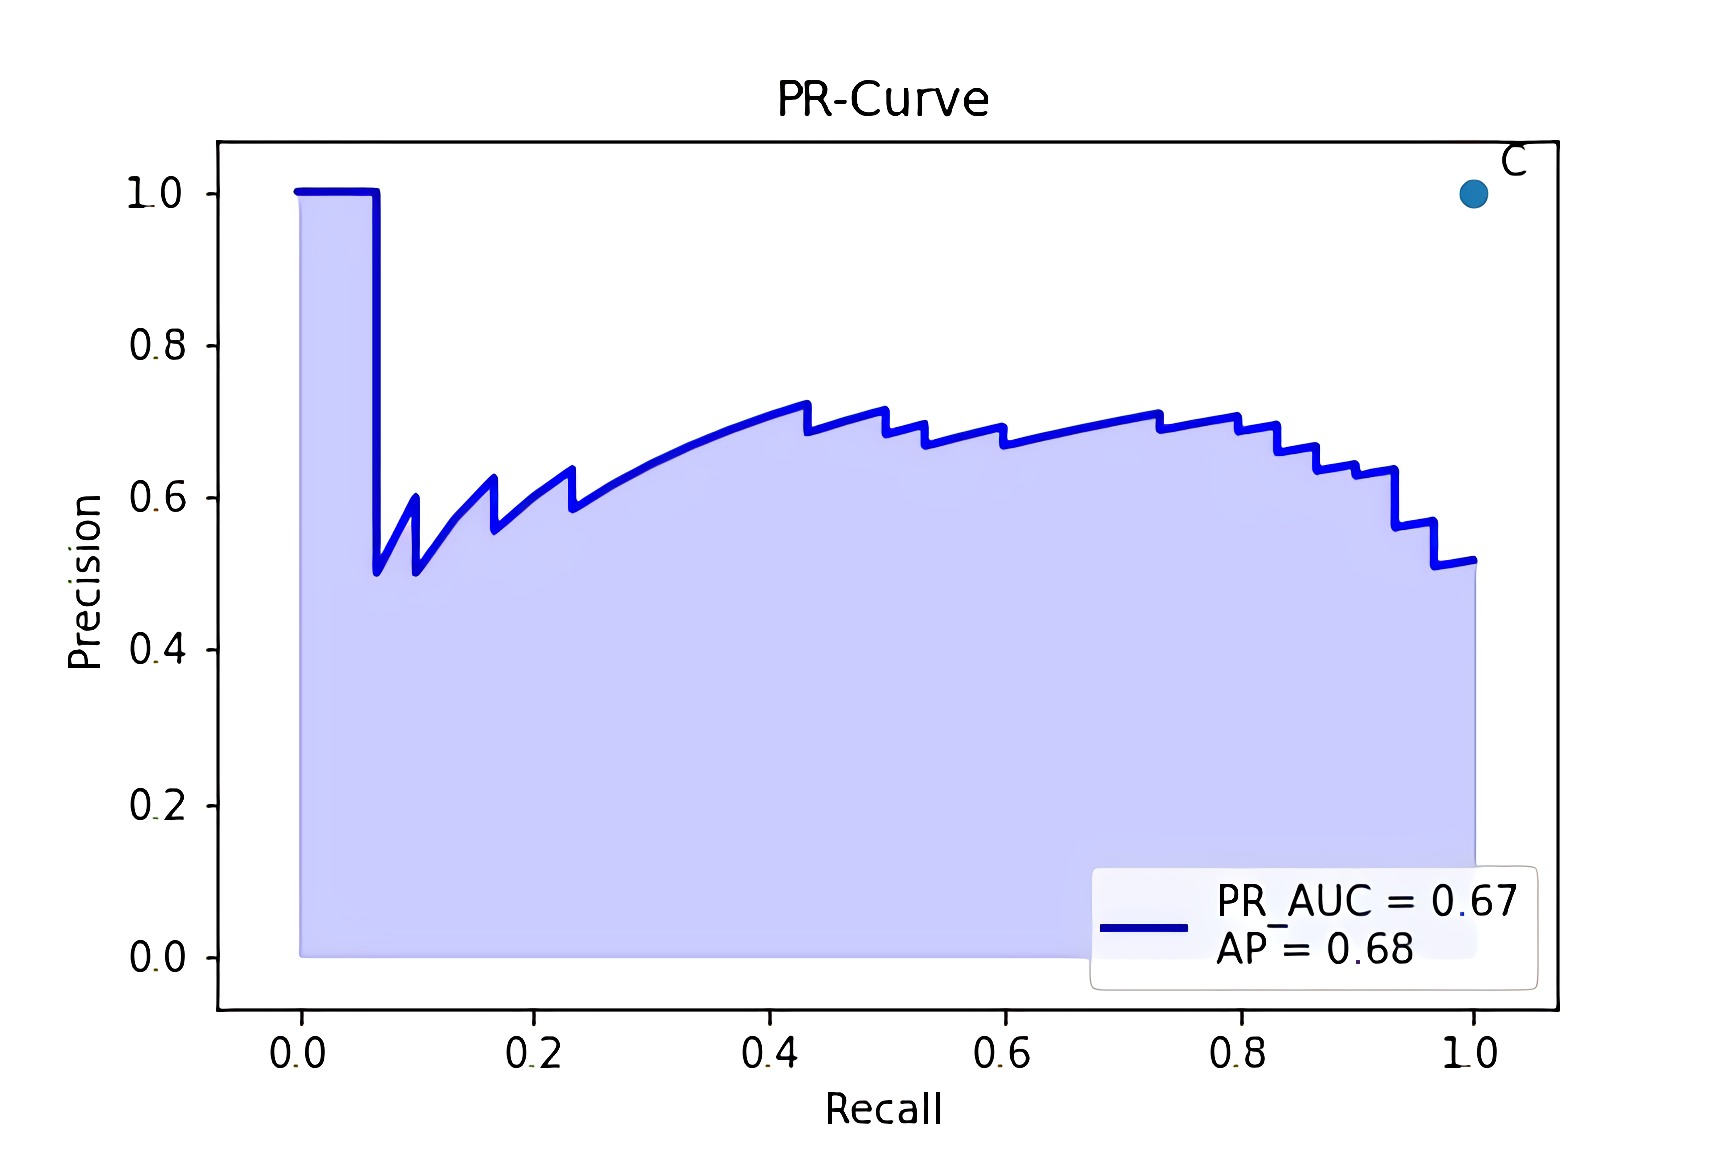
\includegraphics[width=\textwidth]{images/fig5}
        \caption{An example of PR Curve}
        \label{fig5}
    \end{minipage}
    \begin{minipage}{0.49\textwidth}
        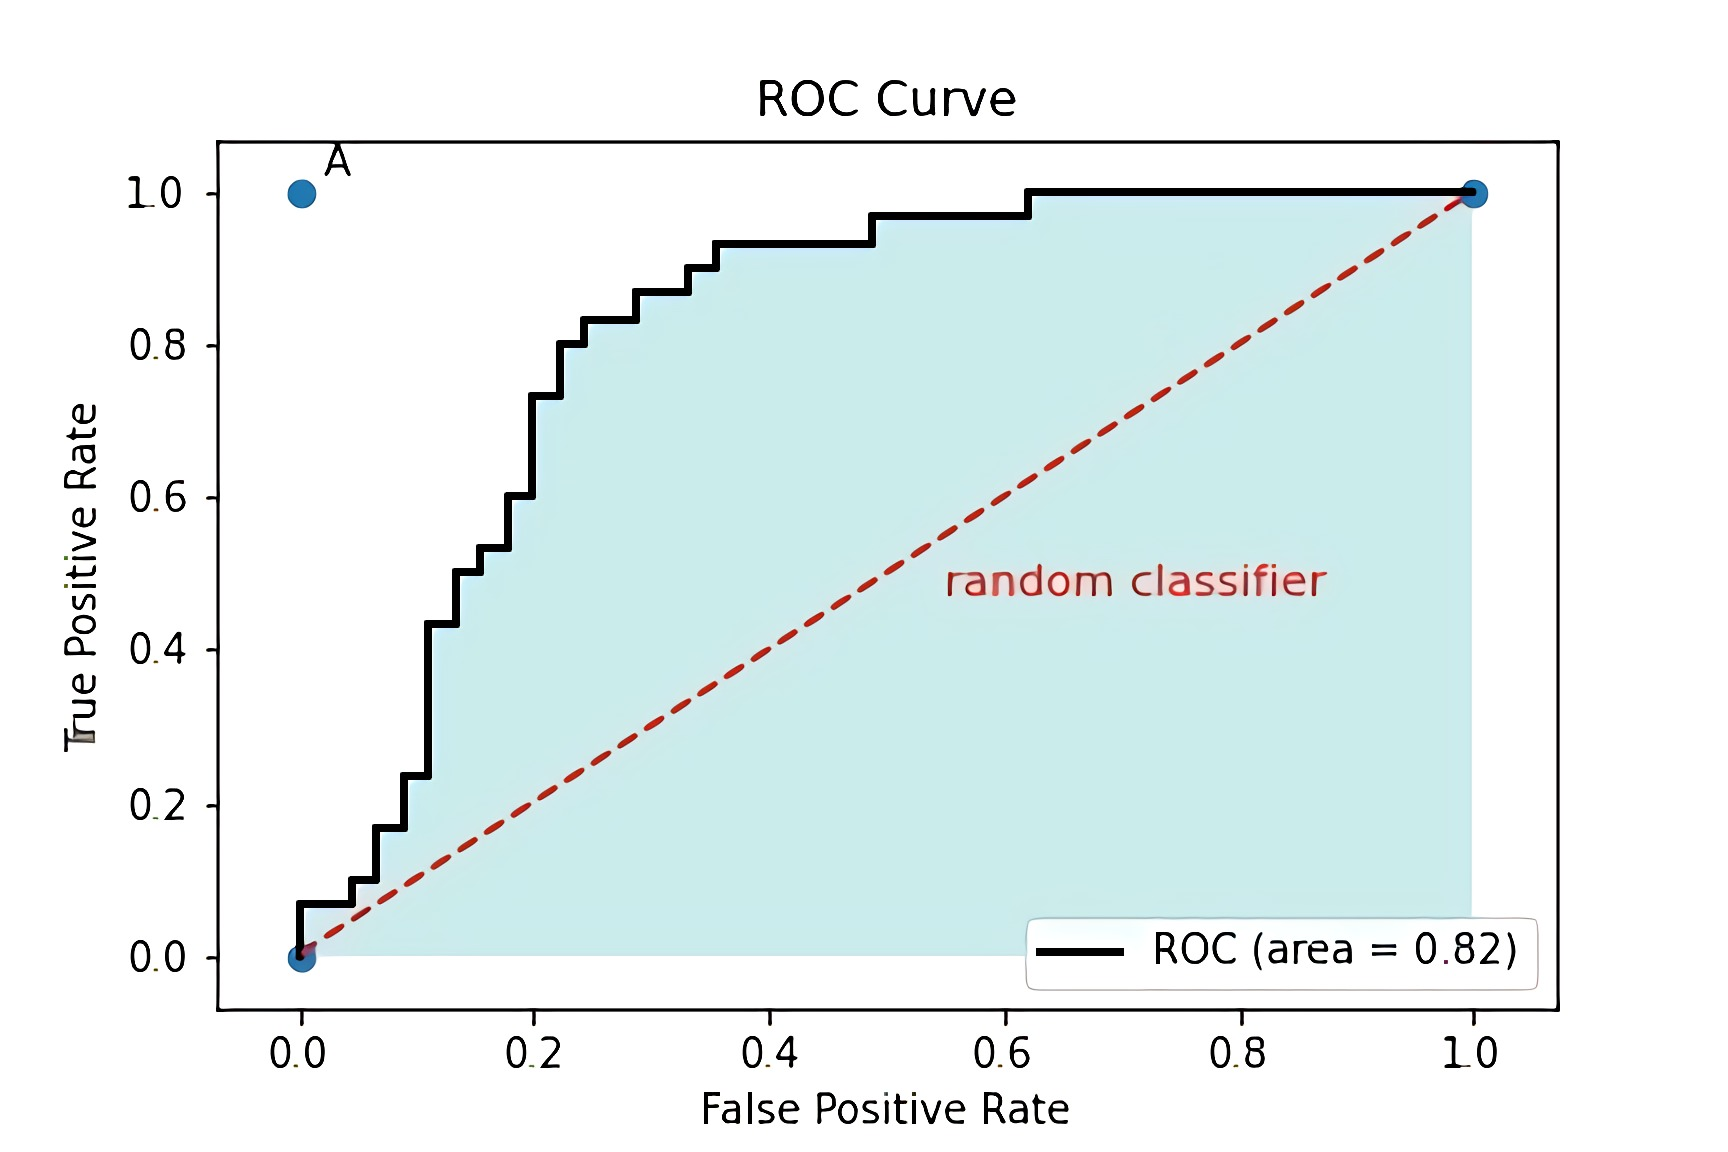
\includegraphics[width=\textwidth]{images/fig6}
        \caption{An example of ROC Curve}
        \label{fig6}
    \end{minipage}
\end{figure}

The ranking metrics focuses on how effectively the base classifiers rank the examples \cite{45}. A numeric score of an example that refers to the probability of being classified as positive is provided by the base classifier, which shows the level of granularity instead of a simple prediction. Different thresholds whose choice affects the trade-offs of both classes' errors can be utilized to test classifiers' performance \cite{10}. \textbf{\textit{Receiver Operating Characteristics (ROC) Curve}} \cite{53} is the most commonly applied ranking metric that is not based on a specific threshold. ROC Curve takes the true positive rate (TPR) and false positive rate (FPR) into account and each point of ROC Curve corresponds to the single classifier performance with a given distribution \cite{17}. The \textbf{\textit{area under the ROC curve (AUCROC)}} is generally applied to measure different classifiers' performance, which is summarized into a single metric \cite{48}. An example of ROC Curve can be observed from Fig \ref{fig6}. Point A $(0,1)$ represents the best performance of the classifier. Therefore, the closer the ROC curve is to A and the more it deviates from the 45-degree diagonal(representing a random classifier), the more successful it is; this also indicates the greater the AUCROC is, the better \cite{53,48}. However, in \cite{17}, it is argued that even a classifier with a high AUCROC can perform poorly in a particular region in ROC space compared with a low AUCROC classifier.

If a dataset is highly skewed, the performance of the algorithm might as observed overly optimistic through a ROC curve \cite{111}. The \textbf{\textit{Precision-Recall (PR) Curve}}, which assesses a more informative representation of performance, is utilized to solve such a limitation \cite{17,54}. PR-Curve is a plot of Recall on the x-axis and Precision on the y-axis \cite{54}, and it can capture the performance of the classifier correctly and effectively if the number of false positives drastically change as the Precision metrics takes the ratio of TP to TP+FP into account \cite{17}. Due to its high level of performances with highly skewed data, it has been applied to the evaluation of performance by many researchers, such as \cite{55,56,57}. Unlike ROC-Curve, whose objective is to be closer to the point $(0,1)$, the highest performing classifier is represented by a PR-Curve residing in the top right of the PR space(point $C(1,1)$) \cite{10}. Similar to AUCROC, the \textbf{\textit{area under the PR Curve (AUCPRC)}} is also a summary of PR-Curve with a single scale value \cite{10}. An example of PR-Curve can be observed in Fig \ref{fig5}.

Recall, Precision, G-Mean, F1 and AUCPRC are applied to evaluate the algorithms' performance in the following experiment.